\section{Tiến độ dự án}

\begin{longtable}{|p{2cm}|p{4cm}|p{4cm}|p{4cm}|}
\hline
\textbf{Tuần (Sprint)} & \textbf{Lê Ngọc Hiền} & \textbf{Nguyễn Mạnh Hùng} & \textbf{Huỳnh Trần Học Đăng} \\
\hline

\textbf{Tuần 1--2} \newline (8/9 -- 21/9)
&
    $\bullet$ Thiết kế wireframe (Figma) chi tiết
    
    $\bullet$ Thiết kế UI tổng thể
    
    $\bullet$ Tạo khu vực chờ (lobby) cơ bản
&
    $\bullet$ Tích hợp mô hình Player
    
    $\bullet$ Tích hợp mô hình bản đồ
    
    $\bullet$ Xây dựng hệ thống camera
&
    $\bullet$ Wireframe Figma (chụp màn hình)
    
    $\bullet$ Tạo mô hình Thẻ bài (Card model)
    
    $\bullet$ Xây dựng logic thắng/thua
\\
\hline

\textbf{Tuần 3--4} \newline (22/9 -- 5/10)
&
    $\bullet$ Tích hợp UI menu chính
    
    $\bullet$ Tích hợp phòng tùy chỉnh (custom room)
    
    $\bullet$ Tích hợp UI menu khu vực chờ trong game
    
    $\bullet$ Thêm cấu hình trò chơi (GameConfig - cấu hình UI)
&
    $\bullet$ Tích hợp mô hình Thẻ bài
    
    $\bullet$ Tích hợp mô hình Xu
    
    $\bullet$ Xử lý vị trí ngồi
    
    $\bullet$ Xử lý vị trí camera
&
    $\bullet$ Triển khai chức năng chia bài
    
    $\bullet$ Triển khai chức năng chọn bài
    
    $\bullet$ Hoàn thiện logic thắng/thua
\\
\hline

\textbf{Tuần 5--6} \newline (6/10 -- 19/10)
&
    $\bullet$ Tích hợp UI Thông tin Lobby
    
    $\bullet$ Xây dựng hệ thống hoạt ảnh UI
    
    $\bullet$ Cải thiện Lobby (đá người chơi, đấu nhanh - quick match)
&
    $\bullet$ Triển khai chức năng dùng bài
    
    $\bullet$ Điều chỉnh camera khi dùng bài
    
    $\bullet$ Tích hợp mô hình Thẻ bài và Bàn chơi (Board)
&
    $\bullet$ Triển khai chức năng phát bài (deal card)
    
    $\bullet$ Triển khai chức năng rút bài (draw card)
    
    $\bullet$ Triển khai thẻ chức năng (action card)
    
    $\bullet$ Triển khai hệ thống Xu
    
    $\bullet$ Triển khai điều kiện thắng
\\
\hline

\textbf{Tuần 7--8} \newline (20/10 -- 9/11)
&
    $\bullet$ UI thay đổi thông tin người chơi
    
    $\bullet$ UI đổi tên Lobby
    
    $\bullet$ Thêm biểu tượng người chơi (icon player)
    
    $\bullet$ Hoàn thiện UI kết thúc game
&
    $\bullet$ Triển khai hoạt ảnh di chuyển đầu người chơi
    
    $\bullet$ Thêm hoạt ảnh sắp xếp chỗ ngồi 
    
    $\bullet$ Đồng bộ hóa (Sync) dữ liệu bàn chơi
    
    $\bullet$ Sửa lỗi chỗ ngồi và hiển thị
&    
    $\bullet$ Sửa lỗi dùng thẻ bài
    
    $\bullet$ Sửa lỗi đồng bộ hóa thẻ bài
    
    $\bullet$ Thêm đồng hồ đếm ngược theo lượt
\\
\hline

\textbf{Tuần 9--10} \newline (10/11 -- 30/11)
&
    $\bullet$ Xây dựng Hệ thống Âm thanh (Audio system)
    
    $\bullet$ Thêm hiệu ứng âm thanh (SFX) và nhạc nền
    
    $\bullet$ Thêm UI Cài đặt cho âm thanh
    
    $\bullet$ Triển khai Trò chuyện bằng giọng nói (Voice chat - Vivox)
    
    $\bullet$ Hỗ trợ chơi khác mạng
&
    $\bullet$ Cải thiện ánh sáng trong game scene
    
    $\bullet$ Highlight đường đi theo vai trò (role)
    
    $\bullet$ Cải thiện di chuyển camera
&
    $\bullet$ Thêm Hiệu ứng hình ảnh (VFX) (thắng/thua, xu, bài chức năng)
    
    $\bullet$ Sửa lỗi liên quan tới thẻ bài và hiệu ứng
\\
\hline

\textbf{Tuần 11--12} \newline (1/12 -- 14/12)
&
    $\bullet$ Viết báo cáo tổng hợp
    
    $\bullet$ Chuẩn bị slide thuyết trình
&
    $\bullet$ Viết báo cáo tổng hợp
    
    $\bullet$ Chuẩn bị slide thuyết trình
&
    $\bullet$ Viết báo cáo tổng hợp
    
    $\bullet$ Chuẩn bị slide thuyết trình
\\
\hline

\textbf{Tuần 13--14} \newline (15/12 -- 28/12)
&
    $\bullet$ Nghiên cứu phát triển giai đoạn 2

    $\bullet$ Sửa lỗi tồn đọng
&
    $\bullet$ Nghiên cứu phát triển giai đoạn 2

    $\bullet$ Sửa lỗi tồn đọng
&
    $\bullet$ Nghiên cứu phát triển giai đoạn 2

    $\bullet$ Sửa lỗi tồn đọng
\\
\hline
\caption{Phân công nhiệm vụ giai đoạn 1 theo Sprint}
\end{longtable}

Trải qua quá trình phát triển 14 tuần của giai đoạn 1, dưới đây là 1 số ảnh chụp màn hình gameplay hiện tại của nhóm:

\begin{figure}[H]
    \centering
    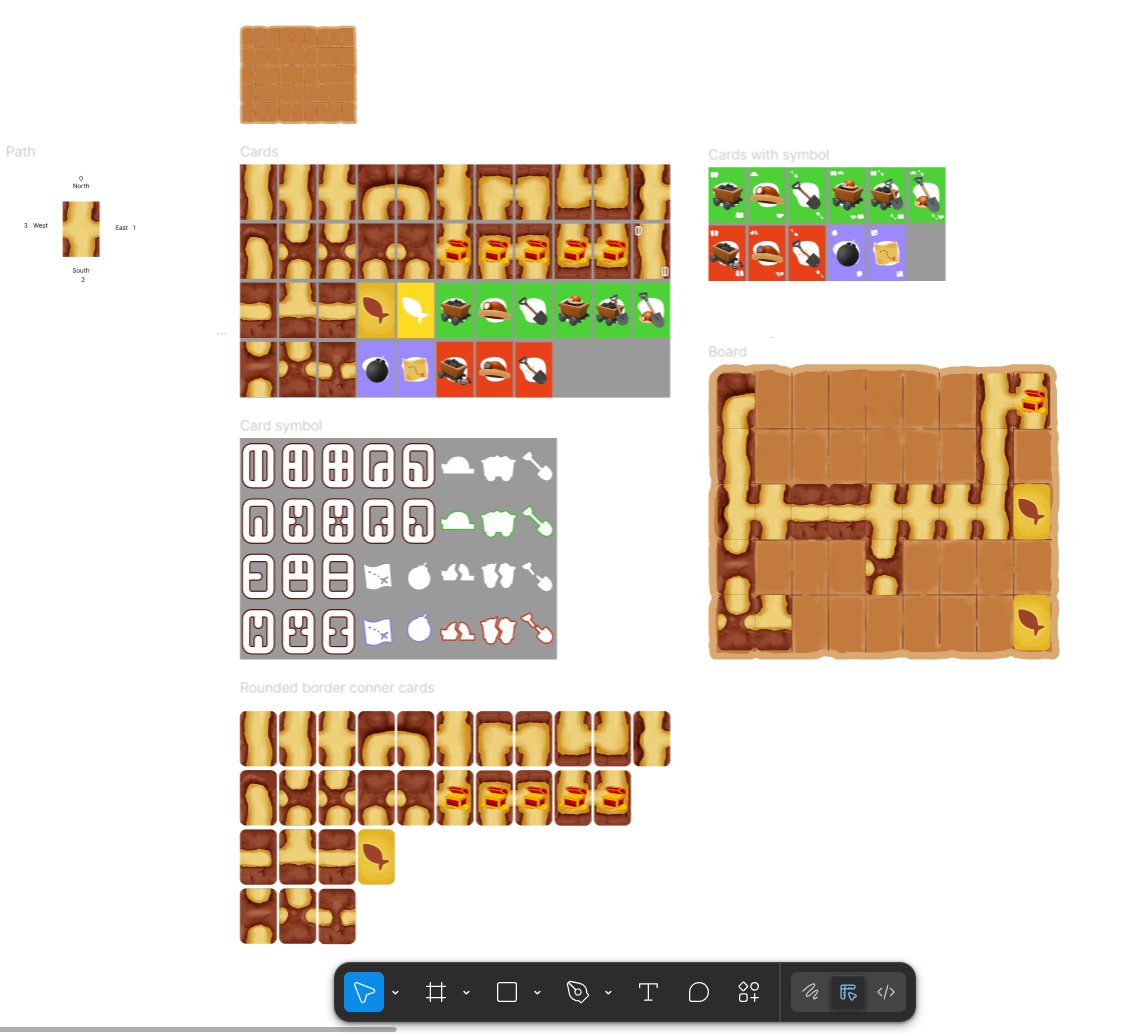
\includegraphics[width=0.75\linewidth]{8. Các thành tựu đạt được/images/CardArts.png}
    \caption{Figma: Bộ thiết kế card}
    \label{fig:placeholder}
\end{figure}

\begin{figure}[H]
    \centering
    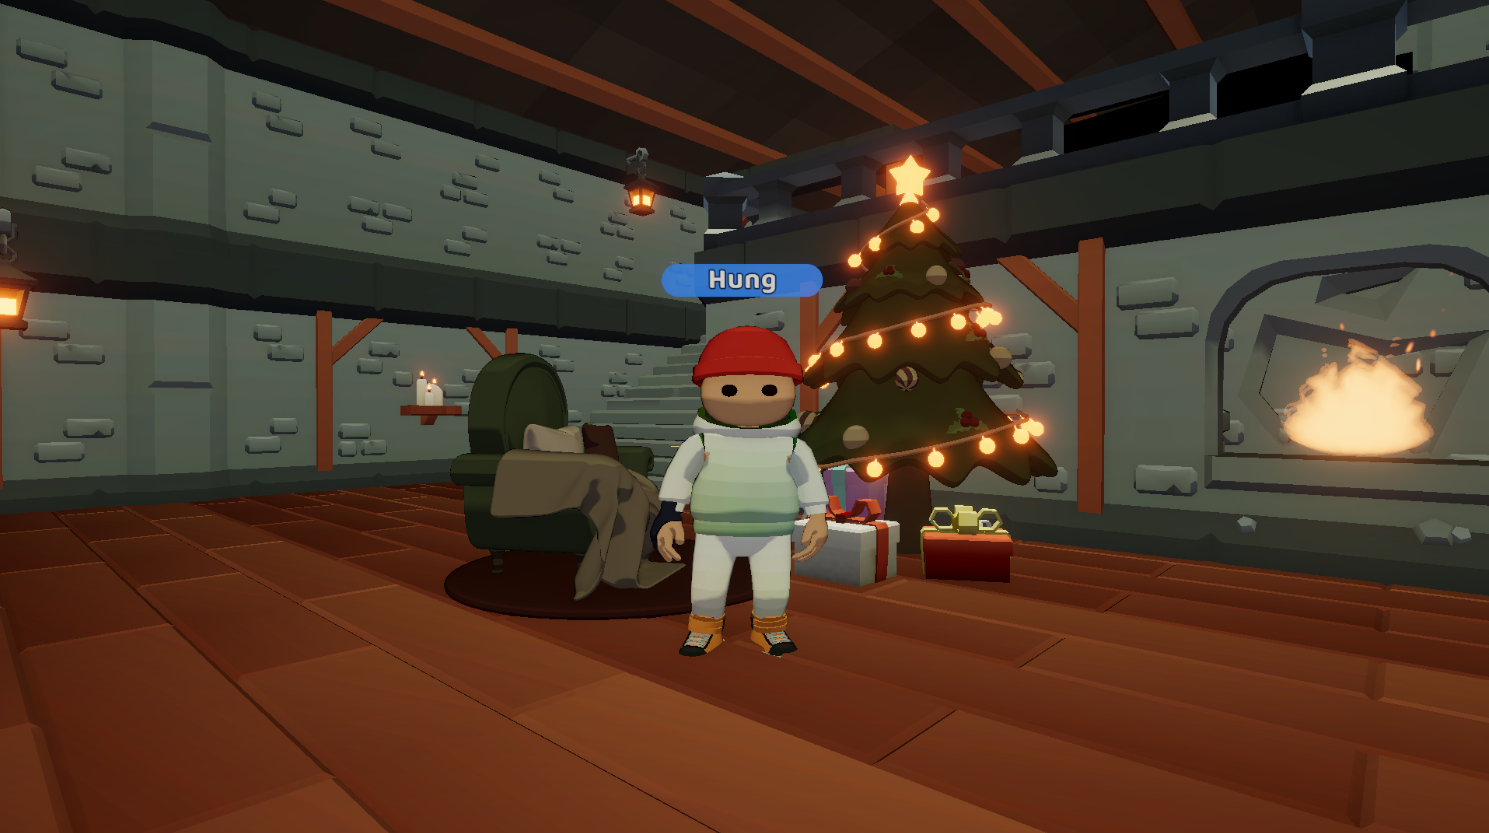
\includegraphics[width=0.75\linewidth]{8. Các thành tựu đạt được/images/character.png}
    \caption{Game Screenshot: Nhân vật khi mới tham gia vào Cabin}
    \label{fig:placeholder}
\end{figure}


\begin{figure}[H]
    \centering
    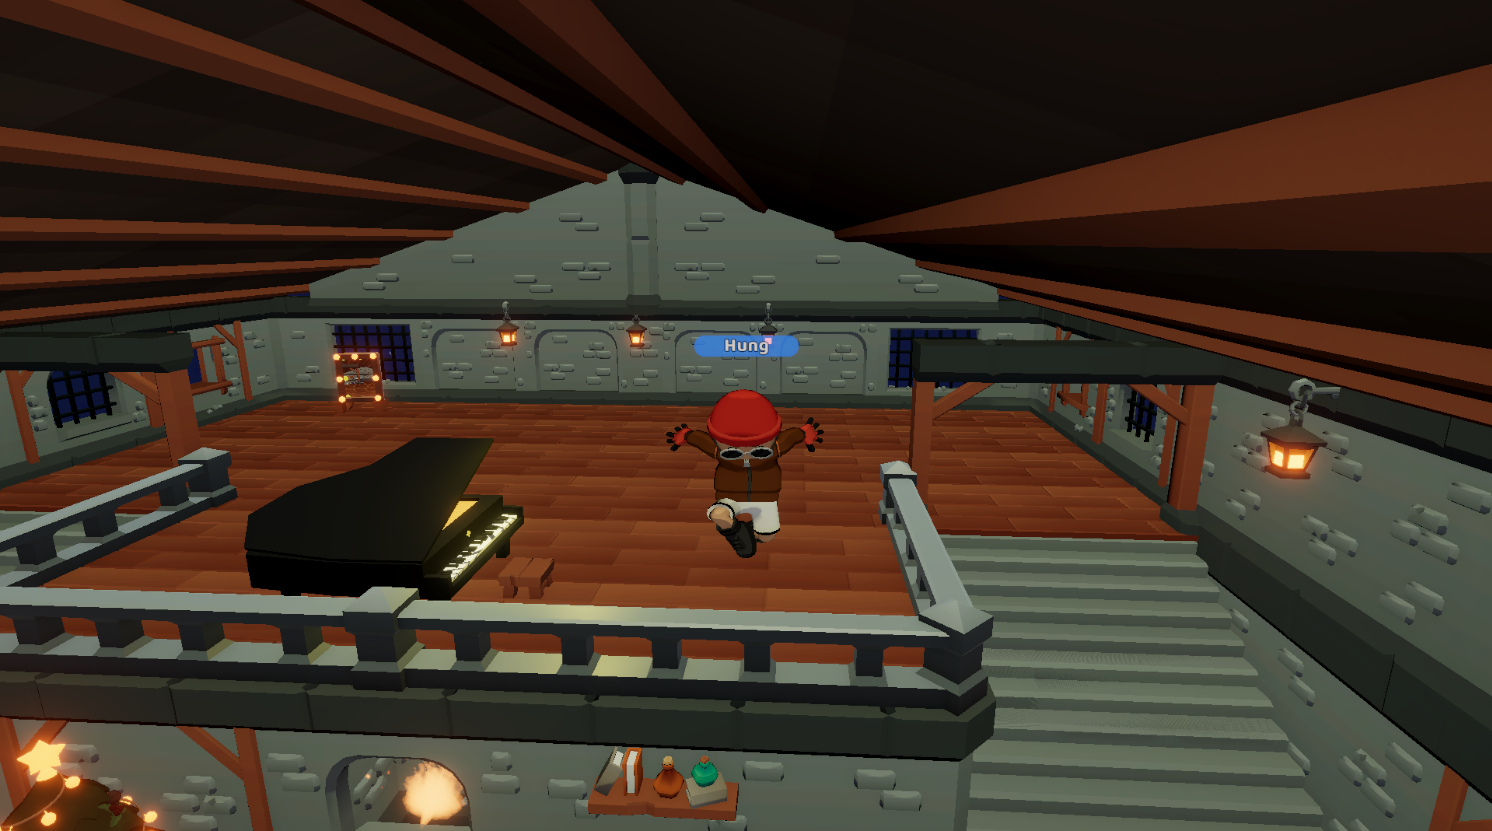
\includegraphics[width=0.75\linewidth]{8. Các thành tựu đạt được/images/jump.png}
    \caption{Game Screenshot: Người chơi nhảy từ gác xuống tầng 1}
    \label{fig:placeholder}
\end{figure}

\begin{figure}[H]
    \centering
    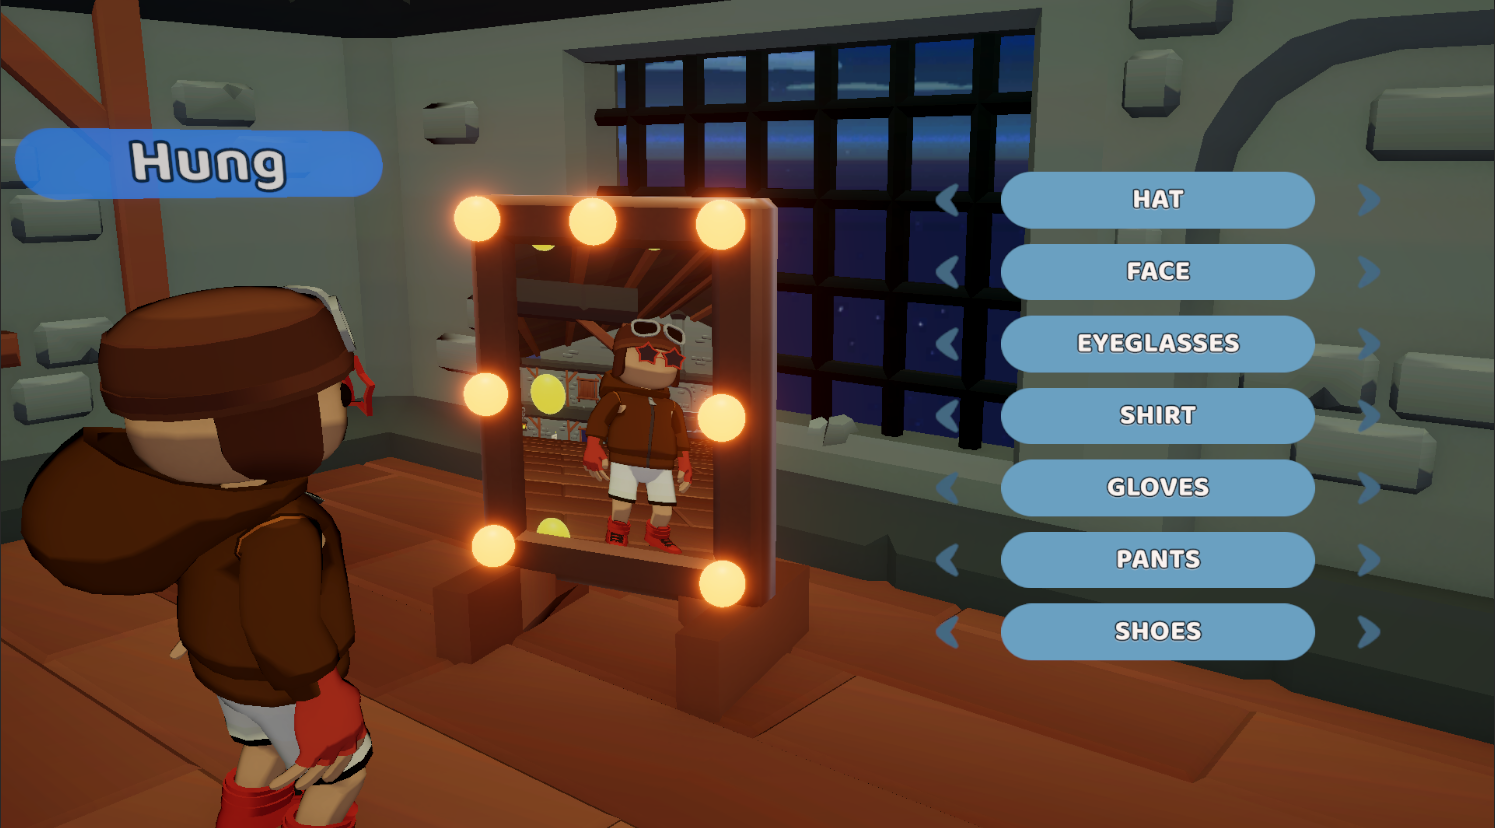
\includegraphics[width=0.75\linewidth]{8. Các thành tựu đạt được/images/mirror.png}
    \caption{Game Screenshot: Người chơi đứng trước gương thay đổi trang phục}
    \label{fig:placeholder}
\end{figure}

\begin{figure}[H]
    \centering
    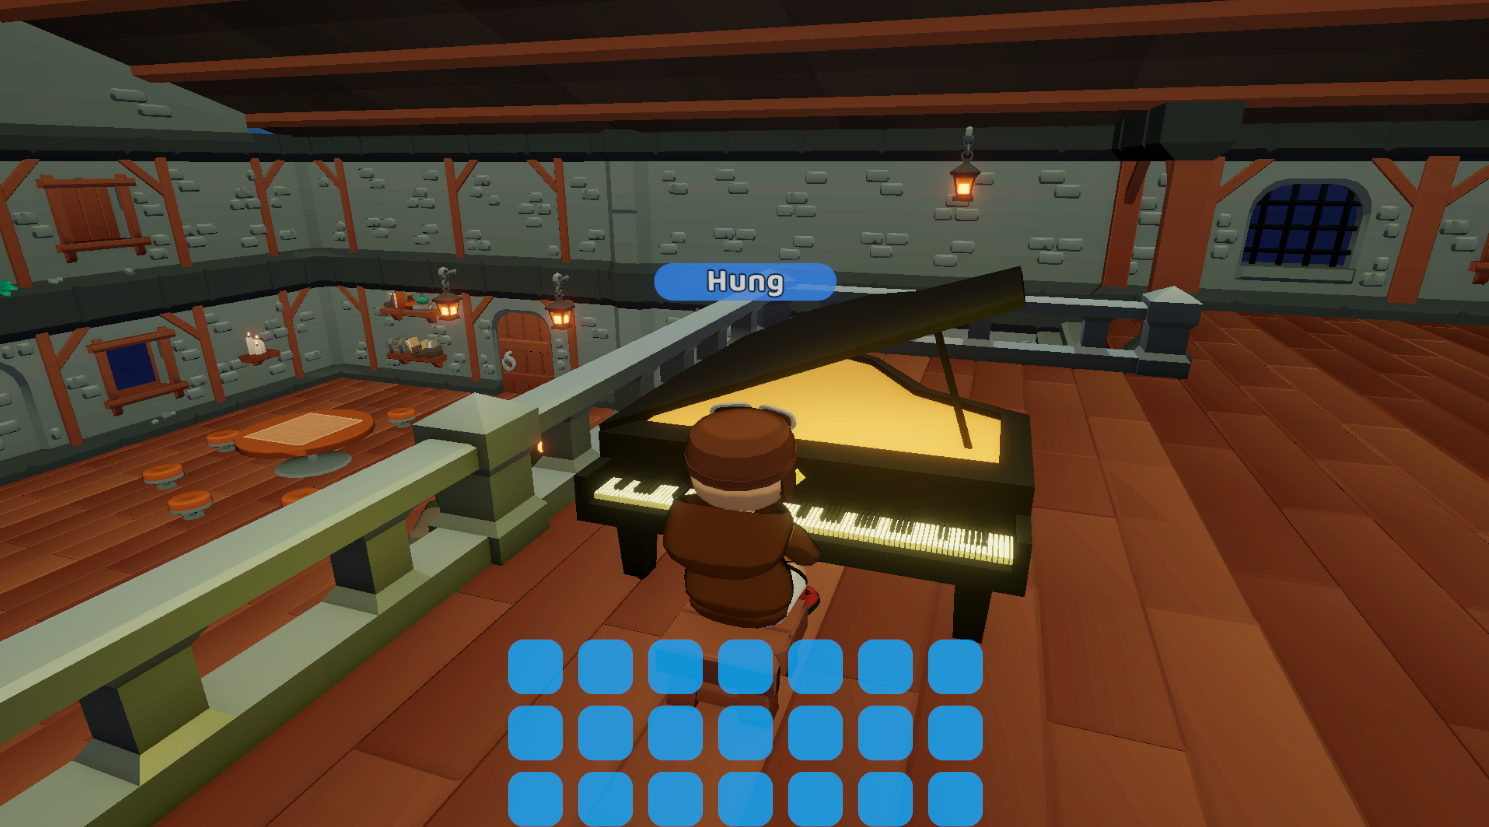
\includegraphics[width=0.75\linewidth]{8. Các thành tựu đạt được/images/piano.png}
    \caption{Game Screenshot: Người chơi chơi đàn piano bằng bàn phím}
    \label{fig:placeholder}
\end{figure}

\begin{figure}[H]
    \centering
    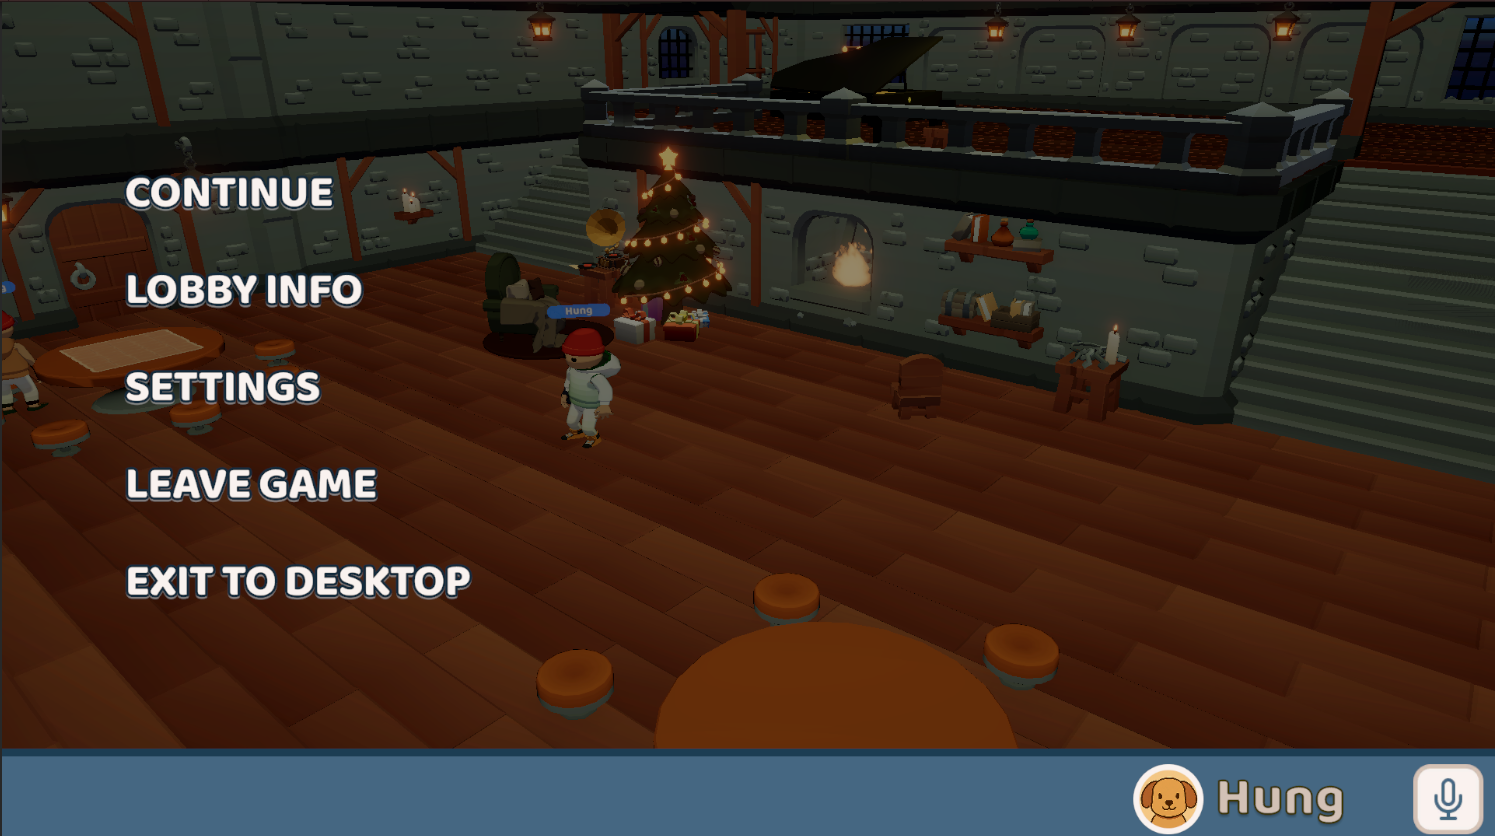
\includegraphics[width=0.75\linewidth]{8. Các thành tựu đạt được/images/ingame-menu.png}
    \caption{Game Screenshot: Menu trong game}
    \label{fig:placeholder}
\end{figure}

\begin{figure}[H]
    \centering
    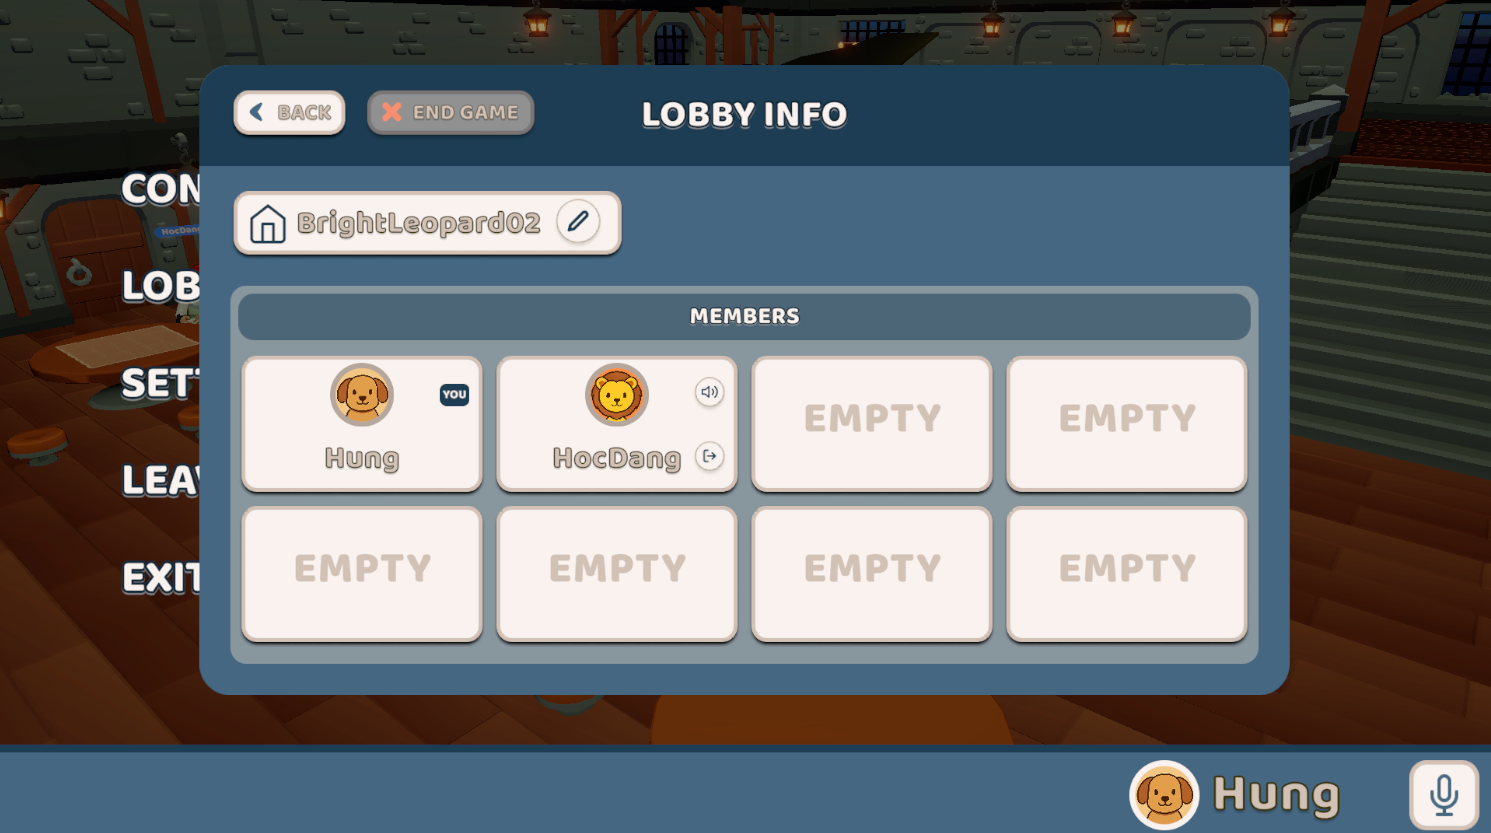
\includegraphics[width=0.75\linewidth]{8. Các thành tựu đạt được/images/lobby-info.png}
    \caption{Game Screenshot: Quản lý lobby, có thể đổi tên phòng, kick người chơi,..}
    \label{fig:placeholder}
\end{figure}

\begin{figure}[H]
    \centering
    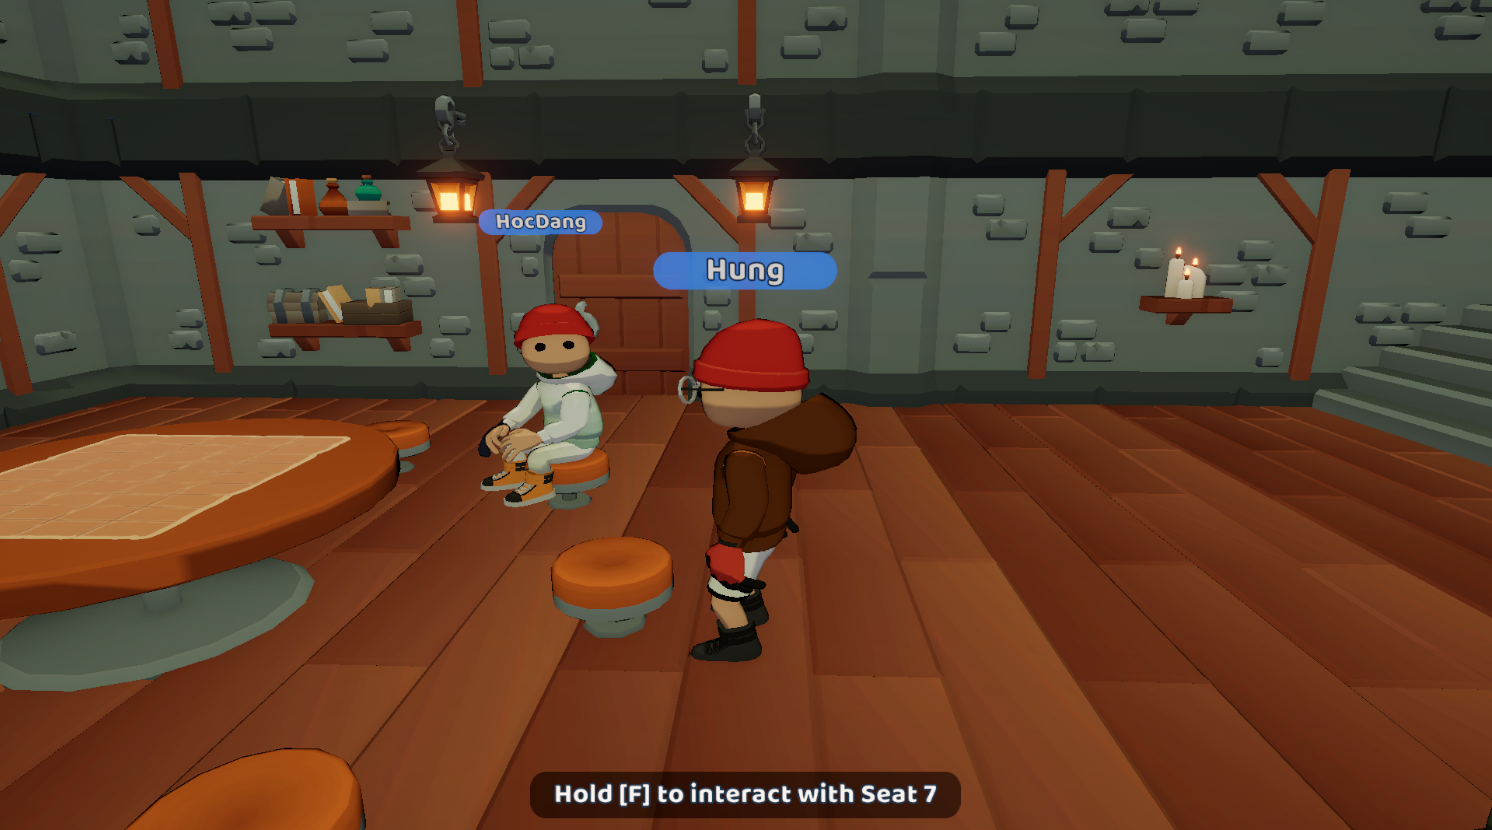
\includegraphics[width=0.75\linewidth]{8. Các thành tựu đạt được/images/interact.png}
    \caption{Game Screenshot: Tương tác với vật thể khi tới gần}
    \label{fig:placeholder}
\end{figure}

\begin{figure}[H]
    \centering
    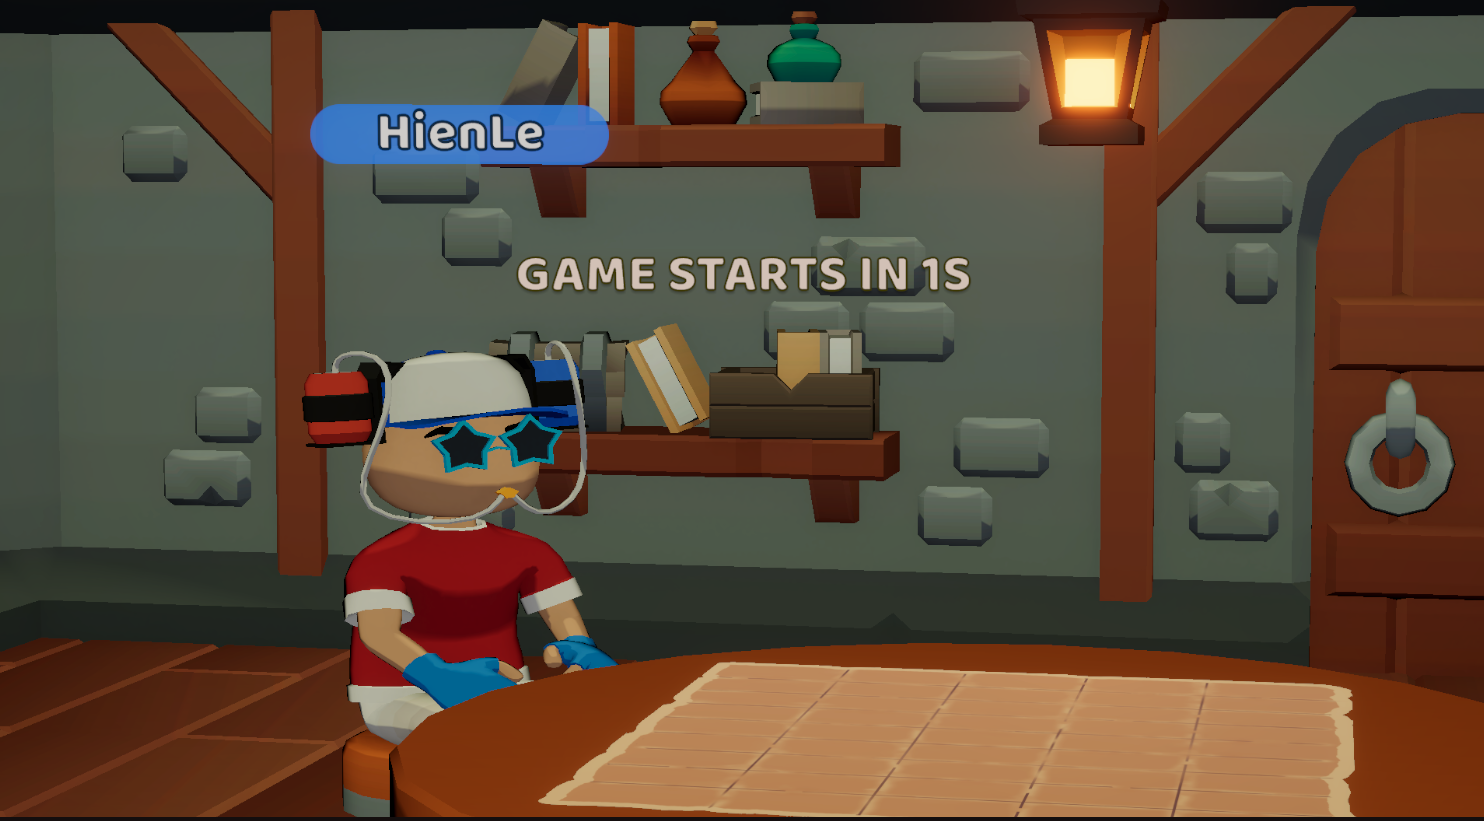
\includegraphics[width=0.75\linewidth]{8. Các thành tựu đạt được/images/start-game.png}
    \caption{Game Screenshot: Người chơi quay đầu nhìn xung quanh}
    \label{fig:placeholder}
\end{figure}


\begin{figure}[H]
    \centering
    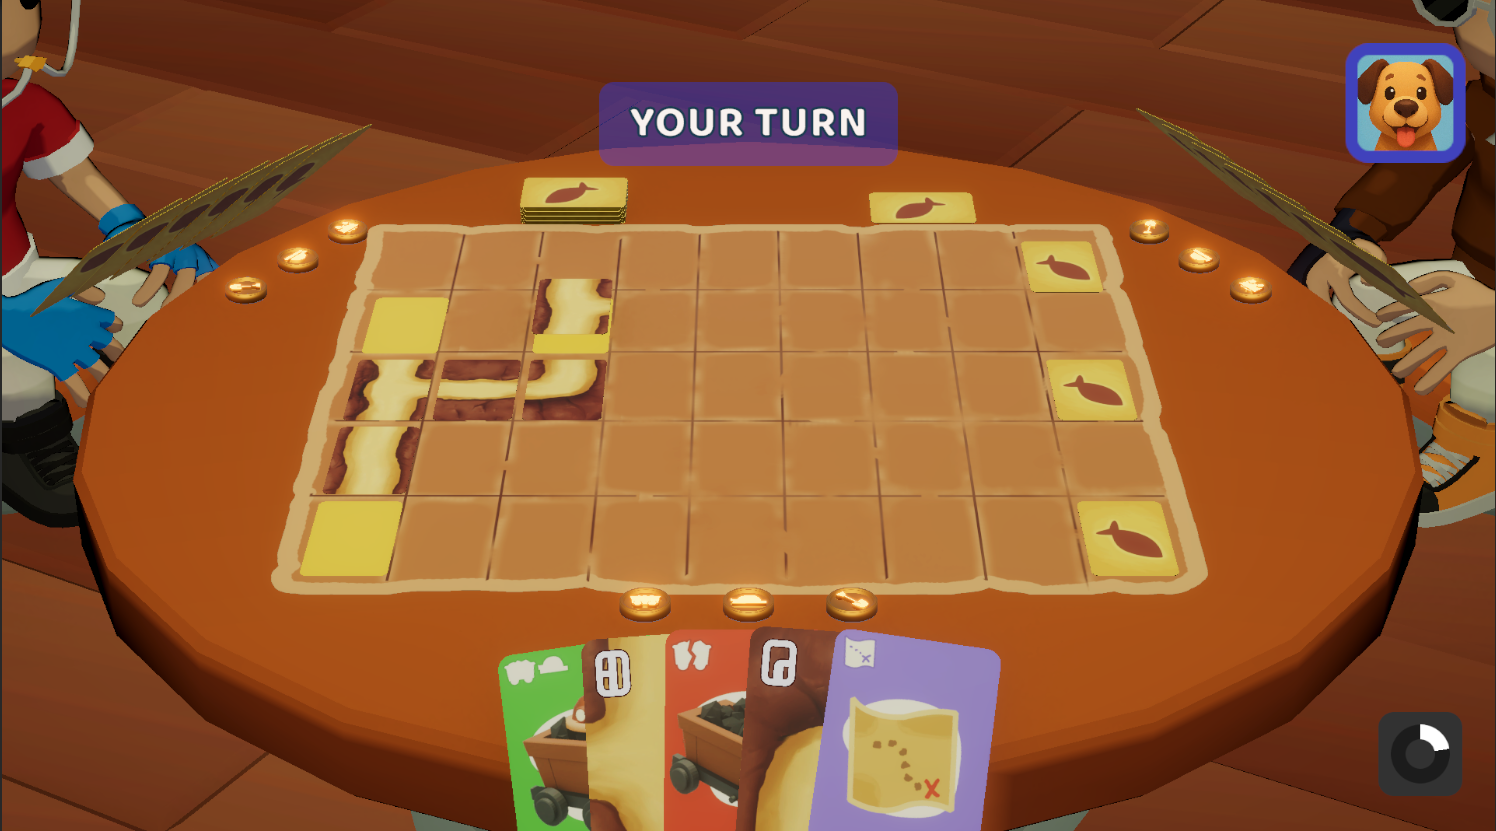
\includegraphics[width=0.75\linewidth]{8. Các thành tựu đạt được/images/playing-card-game.png}
    \caption{Game Screenshot: Khung cảnh của 1 bàn chơi dưới góc nhìn mặc định}
    \label{fig:placeholder}
\end{figure}


\begin{figure}[H]
    \centering
    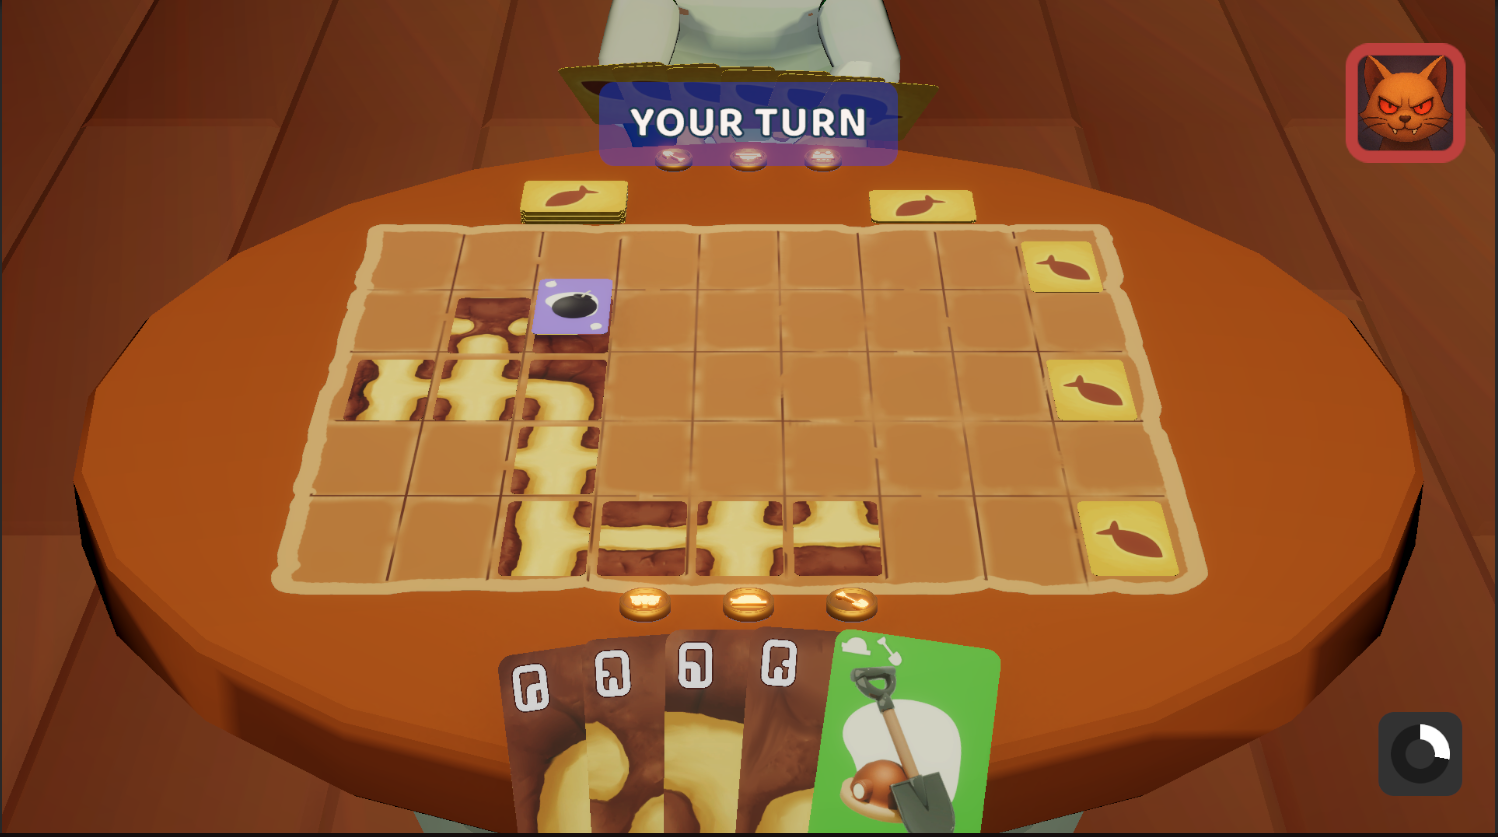
\includegraphics[width=0.75\linewidth]{8. Các thành tựu đạt được/images/bomb.png}
    \caption{Game Screenshot: Sử dụng thể rockfall (bomb) để phá đường}
    \label{fig:placeholder}
\end{figure}


\begin{figure}[H]
    \centering
    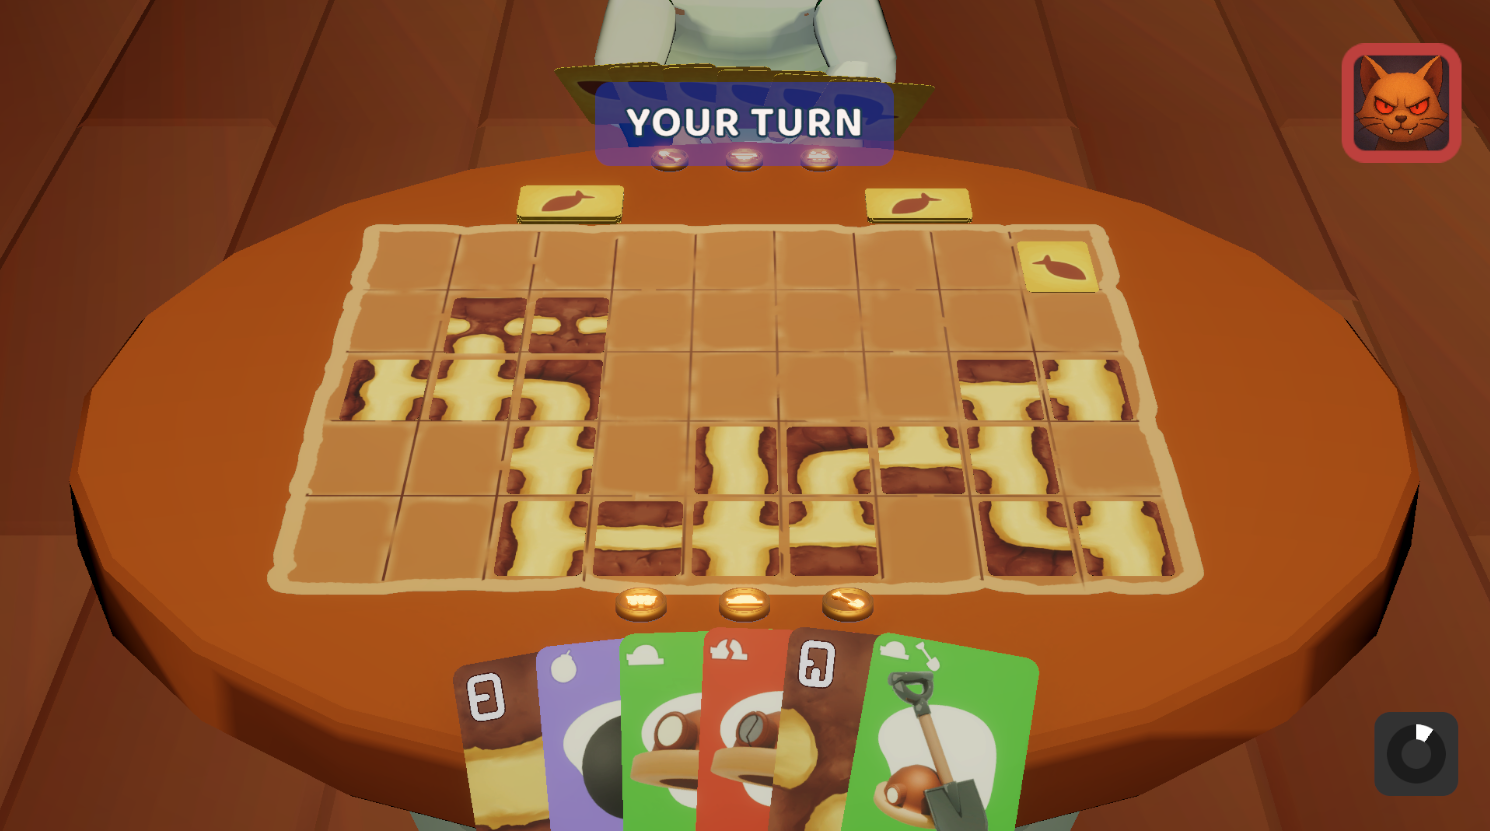
\includegraphics[width=0.75\linewidth]{8. Các thành tựu đạt được/images/empty-goal.png}
    \caption{Game Screenshot: Nối đường tới goal nhưng không chứa vàng}
    \label{fig:placeholder}
\end{figure}

\begin{figure}[H]
    \centering
    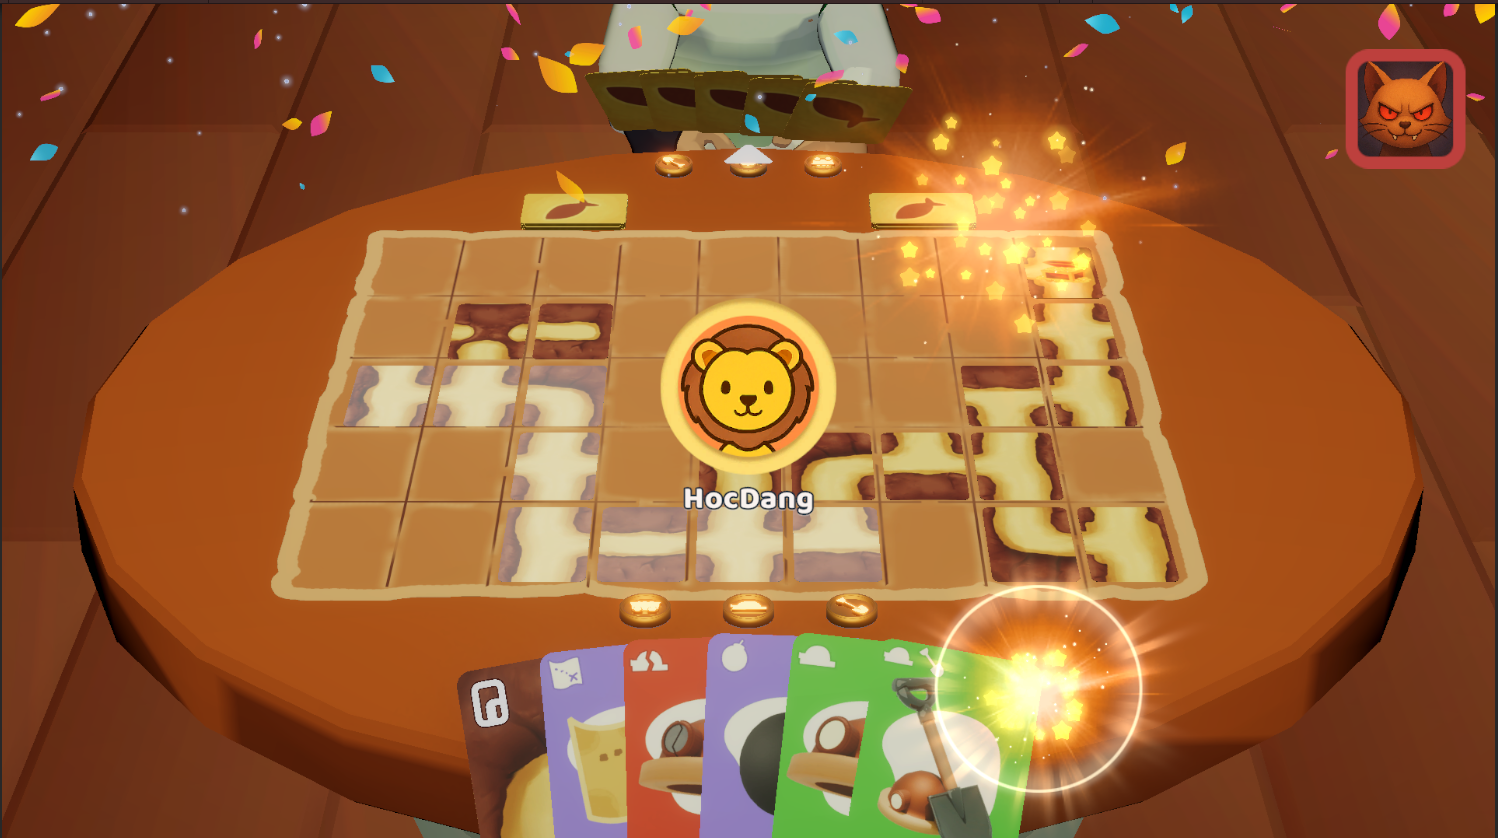
\includegraphics[width=0.75\linewidth]{8. Các thành tựu đạt được/images/end-board-game.png}
    \caption{Game Screenshot: Giao diện thắng/thua khi xong game}
    \label{fig:placeholder}
\end{figure}
